Commençons par donner les définitions et résultats principaux des extensions
rationnelles des fonctions de parking et des chemins de Dyck.

\subsection{Fonctions de parking rationnelles}

Cette partie est illustrée par les exemples 17 à 19 de l'annexe C.

\begin{definition}[a, b - Fonction de Parking]
    Une \emph{a, b - fonction de parking} est une séquence d'entiers
    positifs $(a_1, a_2, \ldots, a_n)$ telle que :\\
    \begin{itemize*}
        \item $n = a$\\
        \item son tri croissant $(b_1, b_2, \ldots, b_n)$ respecte la
        condition suivante :$b_i \leqslant \frac{b}{a}(i-1) + 1$ 
        pour tout $i \leqslant n$.
    \end{itemize*}
\end{definition}

On note $\mathcal{PF}_{a,b}$ l'ensemble des a, b - fonctions de parking.
La formule comptant le nombre d'éléments de cette ensemble est similaire
à celle pour $\mathcal{PF}_{n}$.

\begin{theorem}[Armstrong, Loehr et Warrington, 2014]
    Soit $pf_{a,b}$ le cardinal de $\mathcal{PF}_{a,b}$.
    Nous avons $$pf_{a,b} = b^{a-1}$$
\end{theorem}

\begin{rem}
Le cas classique peut être vu comme le cas $a = n, b = n + 1$.
Autrement dit, $\mathcal{PF}_{n, n + 1} = \mathcal{PF}_n$.
\end{rem}

Similairement au cas classique, on définit une fonction de parking
\emph{rationnelle primitive} comme une fonction de parking primitive
triée en ordre croissant.
On note $\mathcal{PF'}_{a,b}$ l'ensemble des a, b - fonctions de parking
primitives.

\begin{theorem}
    Soit $pf'_{a,b}$ le cardinal de $\mathcal{PF'}_{a,b}$.
    Nous avons $$\displaystyle pf'_{a,b} = 
    \frac{1}{a + b} \binom{a + b}{b}$$
\end{theorem}

Ce nombre est appelé le \emph{nombre de Catalan rationnel}, et on le note
$Cat(a,b)$.
Là aussi, le cas classique correspond à $a = n, b = n + 1$.
Autrement dit, $\mathcal{PF'}_{n, n + 1} = \mathcal{PF'}_n$.

\subsection{Chemins de Dyck rationnels}

Cette partie est illustrée par les exemples 20 à 25 de l'annexe C.

\begin{definition}[a, b - mot de Dyck]
    Un \emph{a, b - mot de Dyck} est un mot $w \in \{0,1\}^*$ tel que :
    \begin{itemize}
        \item pour tout \emph{préfixe} $w'$ de $w$,
            $\displaystyle |w'|_1 \geqslant \frac{a}{b}|w'|_0$.
        \item $|w|_0 = b$.
        \item $|w|_1 = a$.
    \end{itemize}
\end{definition}

Un a, b - mot de Dyck peut être représenté par un chemin allant du point
$(0,0)$ au point $(b,a)$, et restant au dessus de l'axe $y = \frac{a}{b}x$,
appelé \emph{a, b - chemin de Dyck} :
\begin{itemize}
    \item Chaque $1$ correspond à un \emph{pas Nord} $\uparrow$. 
    \item Chaque $0$ correspond à un \emph{pas Est} $\rightarrow$.
\end{itemize}

On note $\mathcal{R}_{a, b}$ l'ensemble des a, b - mots de Dyck.

\begin{theorem}[Bizley (\cite{ref10}), 1954]
    Soit $r_{a,b}$ le cardinal de $\mathcal{R}_{a,b}$.
    Nous avons $$r_{a,b} = \frac{1}{a+b} \binom {a+b}{a} =
    \frac{(a+b-1)!}{a!b!}$$
\end{theorem}

On remarque ainsi que l'on pourra bien créer une bijection entre
$\mathcal{PF'}_{a,b}$ et $\mathcal{R}_{a,b}$.
Cette bijection sera exactement la même que celle entre $\mathcal{PF'}_n$
et $\mathcal{D}_{n}$.

Il reste maintenant à définir les chemins de Dyck qui seront en bijection
avec $\mathcal{PF}_{a,b}$.

\begin{definition}[a, b - mot de Dyck décoré]
    Un \emph{a, b - chemin de Dyck décoré} est un mot $w \in 
    \{0, \ldots, n\}^*$ tel que :
    \begin{itemize}
        \item pour tout préfixe $w'$ de $w$,
            $\displaystyle|w'|_{\neq 0} \geqslant \frac{a}{b}|w'|_0$.
        \item $|w|_0 = b$.
        \item $|w|_{\neq 0} = a$.
        \item pour tout $i \in \{1, \ldots, a\}$, $w$ a exactement une
            occurence de $i$.
        \item si $w_i \neq 0$ et $w_{i+1} \neq 0$,
            alors $w_i < w_{i+1}$. Autrement dit, les labels des pas Nord
            consécutifs sont croissants.
    \end{itemize}
\end{definition}

Un a, b - mot de Dyck décoré peut être représenté par un chemin allant du
point $(0,0)$ au point $(b,a)$, où chaque pas Nord a un label :
\begin{itemize}
    \item Chaque $i \neq 0$ corresponds à un \emph{pas Nord} $\uparrow$
    dont le label est $i$.
    \item Chaque $0$ correspond à un \emph{pas Est} $\rightarrow$.
\end{itemize}

Ces chemins sont appelés \emph{a, b - chemins de Dyck décorés}.\\
On note $\mathcal{LR}_{a,b}$ l'ensemble des a, b - chemins de Dyck.

\begin{theorem}
    Soit $lr_{a,b}$ le cardinal de $\mathcal{LR}_{a,b}$.
    Nous avons $$lr_{a,b} = b^{a - 1}$$.
\end{theorem}

On retrouve bien le même cardinal que pour $\mathcal{PF}_{a,b}$.
A nouveau, la bijection entre $\mathcal{PF}_{a,b}$ et $\mathcal{LR}_{a,b}$
sera exactement la même que celle entre $\mathcal{PF}_n$ et
$\mathcal{LD}_{n}$.

Les relations de couverture restent inchangées :
\begin{itemize}
    \item Pour $\mathcal{PF'}_{a,b}$ et $\mathcal{PF}_{a,b}$ : $\gtrdot$
    \item Pour $\mathcal{R}_{a,b}$ : $\gtrdot_r = \gtrdot_d$
    \item Pour $\mathcal{LR}_{a,b}$ : $\gtrdot_{lr} = \gtrdot_{ld}$ 
\end{itemize}

On peut maintenant construire nos posets pour le cas rationnel.

\subsection{Posets rationnels}

Nous présentons ici une série d'exemple des posets obtenus par les relations
de couverture que nous venons de définir.
Pour le cas primitif comme pour le cas non-primitif, nous étudions un
exemple où $a > b$, et un où $a < b$.
On remarque dans chaque cas que les posets sont bien isomorphes.

\begin{expl}[$a > b$ : Les posets de $\mathcal{R}_{5,3}$ et
    $\mathcal{PF'}_{5,3}$]
    ~\\
    \begin{center}
        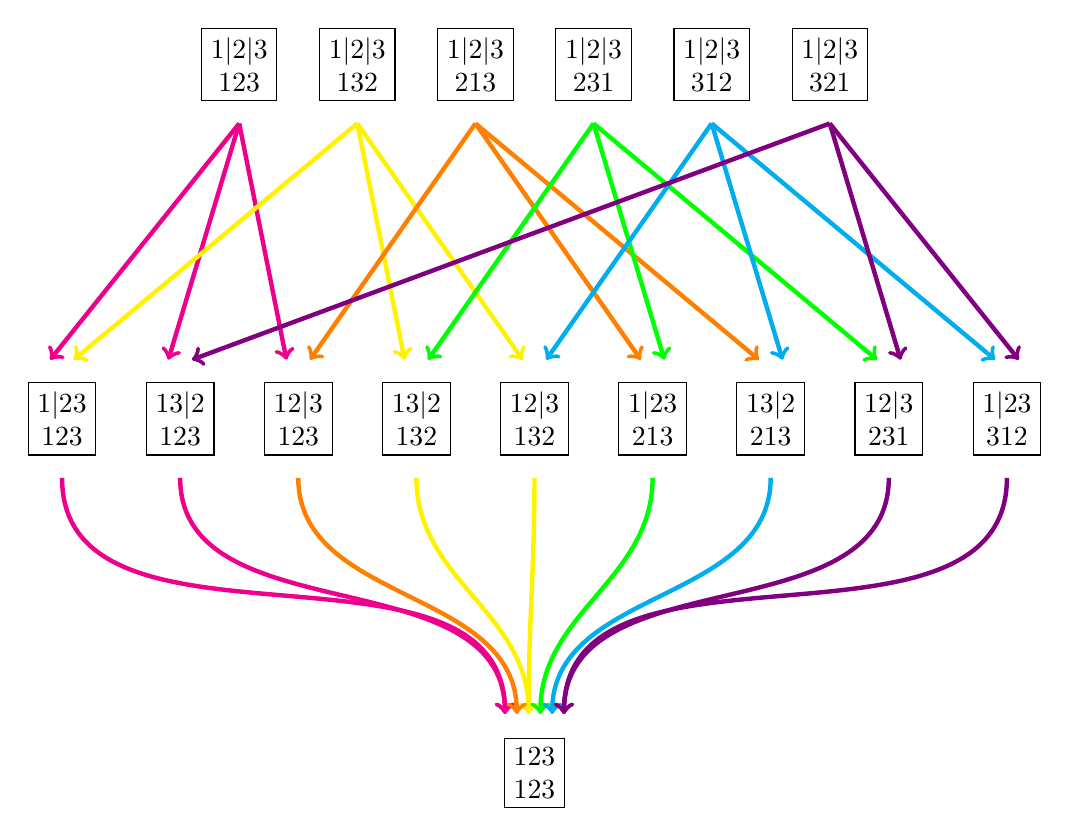
\begin{tikzpicture}[scale = 0.75]
    \node (0)  at (0,0) [align = center]
    [rectangle, draw]
        {$123$\\$123$};
    \node (1)  at (-8,6)[align = center]
    [rectangle, draw]
        {$1|23$\\$123$};
    \node (2)  at (-6,6) [align = center]
    [rectangle, draw]
        {$13|2$\\$123$};
    \node (3)  at (-4,6) [align = center]
    [rectangle, draw]
        {$12|3$\\$123$};
    \node (4)  at (-2,6) [align = center]
    [rectangle, draw]
        {$13|2$\\$132$};
    \node (5)  at (0,6) [align = center]
    [rectangle, draw]
        {$12|3$\\$132$};
    \node (6)  at (2,6) [align = center]
    [rectangle, draw]
        {$1|23$\\$213$};
    \node (7)  at (4,6) [align = center]
    [rectangle, draw]
        {$13|2$\\$213$};
    \node (8)  at (6,6) [align = center]
    [rectangle, draw]
        {$12|3$\\$231$};
    \node (9)  at (8,6) [align = center]
    [rectangle, draw]
        {$1|23$\\$312$};
    \node (10) at (-5,12) [align = center]
    [rectangle, draw]
        {$1|2|3$\\$123$};
    \node (11) at (-3,12) [align = center]
    [rectangle, draw]
        {$1|2|3$\\$132$};
    \node (12) at (-1,12) [align = center]
    [rectangle, draw]
        {$1|2|3$\\$213$};
    \node (13) at (1,12) [align = center]
    [rectangle, draw]
        {$1|2|3$\\$231$};
    \node (14) at (3,12) [align = center]
    [rectangle, draw]
        {$1|2|3$\\$312$};
    \node (15) at (5,12) [align = center]
    [rectangle, draw]
        {$1|2|3$\\$321$};

    \draw [->][color=magenta, ultra thick]
        (-5,11) to (-8.2,7);
    \draw [->][color=magenta, ultra thick]
        (-5,11) to (-6.2, 7); 
    \draw [->][color=magenta, ultra thick]
        (-5,11) to (-4.2,7);
    \draw [->][out=-90,in=90, ultra thick] 
        [color=magenta](-8,5) to (-0.5,1);
    \draw [->][out=-90,in=90, ultra thick] 
        [color=magenta](-6,5) to (-0.5,1);

    \draw [->][color=yellow, ultra thick]
        (-3,11) to (-7.8,7);
    \draw [->][color=yellow, ultra thick]
        (-3,11) to (-2.2,7);
    \draw [->][color=yellow, ultra thick]
        (-3,11) to (-0.2, 7);
    \draw [->][out=-90,in=90, ultra thick] 
        [color=yellow](-2,5) to (-0.1,1);
    \draw [->][out=-90,in=90, ultra thick] 
        [color=yellow](0,5) to (-0.1,1);
    
    \draw [->][color=orange, ultra thick]
        (-1,11) to (1.8,7);
    \draw [->][color=orange, ultra thick]
        (-1,11) to (3.8,7);
    \draw [->][color=orange, ultra thick]
        (-1,11) to (-3.8,7);
    \draw [->][out=-90,in=90, ultra thick] 
        [color=orange](-4,5) to (-0.3,1);

    \draw [->][color=green, ultra thick]
        (1,11) to (2.2,7);
    \draw [->][color=green, ultra thick]
        (1,11) to (-1.8,7);
    \draw [->][color=green, ultra thick]
        (1,11) to (5.8,7);
    \draw [->][out=-90,in=90, ultra thick] 
        [color=green](2,5) to (0.1,1);

    \draw [->][color=cyan, ultra thick]
        (3,11) to (7.8,7);
    \draw [->][color=cyan, ultra thick]
        (3,11) to (4.2,7);
    \draw [->][color=cyan, ultra thick]
        (3,11) to (0.2,7);
    \draw [->][out=-90,in=90, ultra thick] 
        [color=cyan](4,5) to (0.3,1);

    \draw [->][color=violet, ultra thick]
        (5,11) to (8.2,7);
    \draw [->][color=violet, ultra thick]
        (5,11) to (-5.8,7);
    \draw [->][color=violet, ultra thick]
        (5,11) to (6.2,7);
    \draw [->][out=-90,in=90, ultra thick] 
        [color=violet](6,5) to (0.5,1);
    \draw [->][out=-90,in=90, ultra thick] 
        [color=violet](8,5) to (0.5,1);
    
\end{tikzpicture}
        Chacun de ces posets comporte $\frac {1}{8} \binom{8}{5} = 7$
        éléments.
    \end{center}
\end{expl}

\newpage
\begin{expl}[$a < b$ : Les posets de $\mathcal{R}_{3,7}$ et
    $\mathcal{PF'}_{3,7}$]
    ~\\
    \begin{center}
        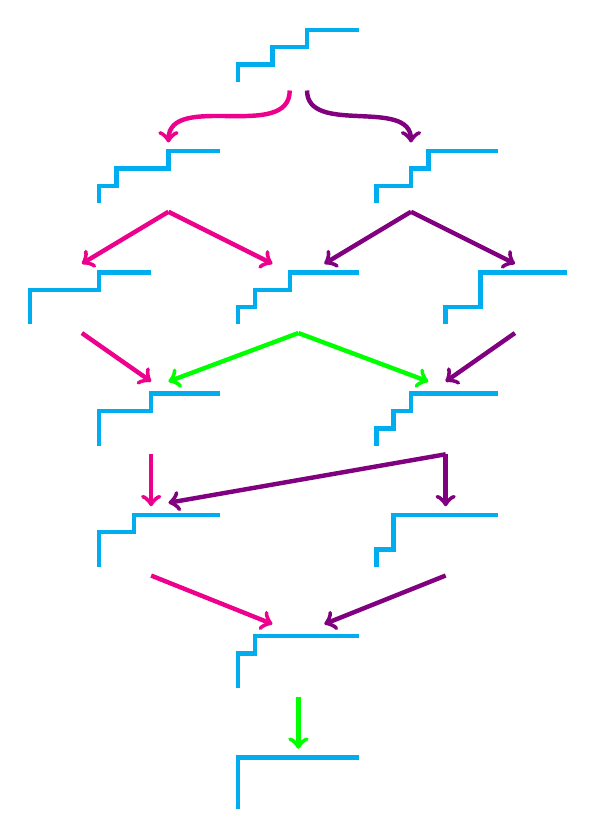
\begin{tikzpicture}[scale = 0.22]
    \draw [ultra thick, color = cyan] (0,0) -- (0,1)
        -- (0,2) -- (0,3) -- (1,3) -- (2,3) -- (3,3)
        -- (4,3) -- (5,3) -- (6,3) -- (7,3);

    \draw [ultra thick, color = cyan] (0,7) -- (0,8)
        -- (0,9) -- (1,9) -- (1,10) -- (2,10) -- (3,10)
        -- (4,10) -- (5,10) -- (6,10) -- (7,10);

    \draw [ultra thick, color = cyan] (-8,14) -- (-8,15)
        -- (-8,16) -- (-7,16) -- (-6,16) -- (-6,17) -- (-5,17)
        -- (-4,17) -- (-3,17) -- (-2,17) -- (-1,17);
        
    \draw [ultra thick, color = cyan] (8,14) -- (8,15)
        -- (9,15) -- (9,16) -- (9,17) -- (10,17)
        -- (11,17) -- (12,17) -- (13,17) -- (14,17)
        -- (15,17);

    \draw [ultra thick, color = cyan] (-8,21) -- (-8,22)
        -- (-8,23) -- (-7,23) -- (-6,23) -- (-5,23)
        -- (-5,24) -- (-4,24) -- (-3,24) -- (-2,24)
        -- (-1, 24);

    \draw [ultra thick, color = cyan] (8,21) -- (8,22)
        -- (9,22) -- (9,23) -- (10,23) -- (10,24) -- (11,24)
        -- (12,24) -- (13,24) -- (14,24) -- (15,24);

    \draw [ultra thick, color = cyan] (-12,28) -- (-12,29)
        -- (-12,30) -- (-11,30) -- (-10,30) -- (-9,30) -- (-8,30)
        -- (-8,31) -- (-7,31) -- (-6,31) -- (-5,31);

    \draw [ultra thick, color = cyan] (0,28) -- (0,29)
        -- (1,29) -- (1,30) -- (2,30) -- (3,30) -- (3,31)
        -- (4,31) -- (5,31) -- (6,31) -- (7,31);

    \draw [ultra thick, color = cyan] (12,28) -- (12,29)
        -- (13,29) -- (14,29) -- (14,30) -- (14,31) -- (15,31)
        -- (16,31) -- (17,31) -- (18,31) -- (19,31);

    \draw [ultra thick, color = cyan] (-8,35) -- (-8,36)
        -- (-7,36) -- (-7,37) -- (-6,37) -- (-5,37) -- (-4,37)
        -- (-4,38) -- (-3,38) -- (-2,38) -- (-1,38);

    \draw [ultra thick, color = cyan] (8,35) -- (8,36)
        -- (9,36) -- (10,36) -- (10,37) -- (11,37) -- (11,38)
        -- (12,38) -- (13,38) -- (14,38) -- (15,38);

    \draw [ultra thick, color = cyan] (0,42) -- (0,43)
        -- (1,43) -- (2,43) -- (2,44) -- (3,44) -- (4,44)
        -- (4,45) -- (5,45) -- (6,45) -- (7,45);

    \draw [->][out=-90,in=90, ultra thick] 
        [color=magenta](3,41.5) to (-4,38.5);
    \draw [->][color=magenta, ultra thick]
        (-4,34.5) to (-9,31.5);
    \draw [->][color=magenta, ultra thick]
        (-4,34.5) to (2,31.5);        
    \draw [->][color=magenta, ultra thick]
        (-9,27.5) to (-5,24.7);
    \draw [->][color=magenta, ultra thick]
        (-5,20.5) to (-5,17.5);
    \draw [->][color=magenta, ultra thick]
        (-5,13.5) to (2,10.7);

    \draw [->][color=green, ultra thick]
        (3.5,27.5) to (-4,24.7);
    \draw [->][color=green, ultra thick]
        (3.5,27.5) to (11,24.7);
    \draw [->][out=-90,in=90, ultra thick] 
        [color=green](3.5,6.5) to (3.5,3.5);

    \draw [->][out=-90,in=90, ultra thick]
        [color=violet](4,41.5) to (10,38.5);
    \draw [->][color=violet, ultra thick]
        (10,34.5) to (5,31.5);
    \draw [->][color=violet, ultra thick]
        (10,34.5) to (16,31.5);
    \draw [->][color=violet, ultra thick]
        (16,27.5) to (12,24.7);
    \draw [->][color=violet, ultra thick]
        (12,20.5) to (-4,17.7);
    \draw [->][color=violet, ultra thick]
        (12,20.5) to (12,17.5);
    \draw [->][color=violet, ultra thick]
        (12,13.5) to (5,10.7);

\end{tikzpicture}
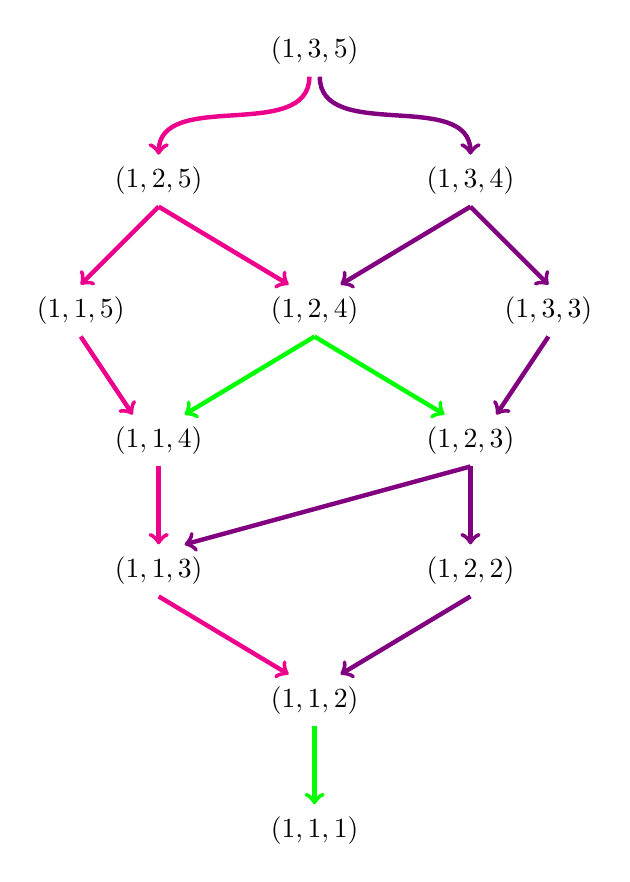
\begin{tikzpicture}[scale = 0.33]
    \node at (0,0) {$(1,1,1)$};

    \node at (0,5) {$(1,1,2)$};

    \node at (-6,10) {$(1,1,3)$};                
    \node at (6,10)  {$(1,2,2)$};

    \node at (-6,15) {$(1,1,4)$};
    \node at (6,15)  {$(1,2,3)$};

    \node at (-9,20) {$(1,1,5)$};
    \node at (0,20)  {$(1,2,4)$};
    \node at (9,20)  {$(1,3,3)$};

    \node at (-6,25) {$(1,2,5)$};
    \node at (6,25)  {$(1,3,4)$};

    \node at (0,30) {$(1,3,5)$};

    \draw [->][out=-90,in=90, ultra thick] 
        [color=magenta](-0.2,29) to (-6,26);
    \draw [->][color=magenta, ultra thick]
        (-6,24) to (-9,21);
    \draw [->][color=magenta, ultra thick]
        (-6,24) to (-1,21);        
    \draw [->][color=magenta, ultra thick]
        (-9,19) to (-7,16);
    \draw [->][color=magenta, ultra thick]
        (-6,14) to (-6,11);
    \draw [->][color=magenta, ultra thick]
        (-6,9) to (-1,6);

    \draw [->][color=green, ultra thick]
        (0,19) to (-5,16);
    \draw [->][color=green, ultra thick]
        (0,19) to (5,16);
    \draw [->][out=-90,in=90, ultra thick] 
        [color=green](0,4) to (0,1);

    \draw [->][out=-90,in=90, ultra thick]
        [color=violet](0.2,29) to (6,26);
    \draw [->][color=violet, ultra thick]
        (6,24) to (1,21);
    \draw [->][color=violet, ultra thick]
        (6,24) to (9,21);
    \draw [->][color=violet, ultra thick]
        (9,19) to (7,16);
    \draw [->][color=violet, ultra thick]
        (6,14) to (-5,11);
    \draw [->][color=violet, ultra thick]
        (6,14) to (6,11);
    \draw [->][color=violet, ultra thick]
        (6,9) to (1,6);

\end{tikzpicture}
~\\
~\\
        Chacun de ces posets comporte $\frac {1}{10} \binom{10}{3} = 12$
        éléments.
    \end{center}
\end{expl}

\begin{expl}[$a > b$ : Les posets de $\mathcal{LR}_{5,2}$ et
    $\mathcal{PF}_{5,2}$]
    ~\\
    \begin{center}
        \begin{center}
    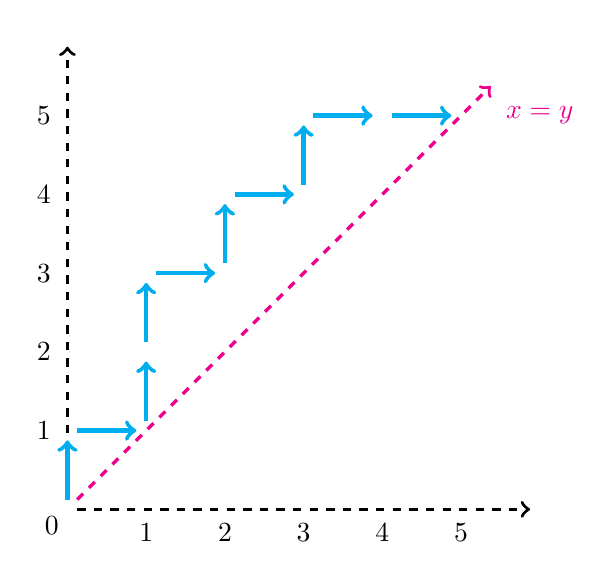
\begin{tikzpicture}[scale=1]
        \node (a) at (0, 0) {};
        \node (b) at (0, 6) {};
        \node (c) at (6, 0) {};
        \node (d) at (5.5, 5.5) {};
        \node (e) at (6, 5) [color = magenta]
            {$x = y$}; 
        \draw [dashed, very thick, ->] (a) to (b);
        \draw [dashed, very thick, ->] (a) to (c);
        \draw [dashed, very thick, ->]
            [color = magenta] (a) to (d);

        \node (1)  at (0,0)   {};
        \node (2)  at (0,1)   {};
        \node (3)  at (1,1)   {};
        \node (4)  at (1,2)   {};
        \node (5)  at (1,3)   {};
        \node (6)  at (2,3)   {};
        \node (7)  at (2,4)   {};
        \node (8)  at (3,4)   {};
        \node (9)  at (3,5)   {};
        \node (10) at (4,5)   {};
        \node (11) at (5,5)   {};
        \draw [->, ultra thick, color = cyan]
            (1)  to (2);
        \draw [->, ultra thick, color = cyan] 
            (2)  to (3);
        \draw [->, ultra thick, color = cyan]
            (3)  to (4);
        \draw [->, ultra thick, color = cyan]
            (4)  to (5);
        \draw [->, ultra thick, color = cyan]
            (5)  to (6);
        \draw [->, ultra thick, color = cyan]
            (6)  to (7);
        \draw [->, ultra thick, color = cyan]
            (7)  to (8);
        \draw [->, ultra thick, color = cyan]
            (8)  to (9);
        \draw [->, ultra thick, color = cyan]
            (9)  to (10);
        \draw [->, ultra thick, color = cyan]
            (10) to (11);

        \node at (-0.2, -0.2) {$0$};
        \node at (-0.3, 1)    {$1$};
        \node at (1, -0.3)    {$1$};
        \node at (-0.3, 2)    {$2$};
        \node at (2, -0.3)    {$2$};
        \node at (-0.3, 3)    {$3$};
        \node at (3, -0.3)    {$3$};
        \node at (-0.3, 4)    {$4$};
        \node at (4, -0.3)    {$4$};
        \node at (-0.3, 5)    {$5$};
        \node at (5, -0.3)    {$5$};

    \end{tikzpicture}
\end{center}
        Pour plus de clarté, les flêches ont été simplifiées.
        Celles des deux plus hauts niveaux sont à comprendre ainsi :
        chaque flêche finit là ou il y a une croix de la même couleur.
        Il y a  $2^4 = 16$ éléments dans chacun de ces posets.
    \end{center}
\end{expl}


\begin{expl}[$a < b$ : Les posets de $\mathcal{LR}_{2,7}$ et
    $\mathcal{PF}_{2,7}$]
    ~\\
    \begin{center}
        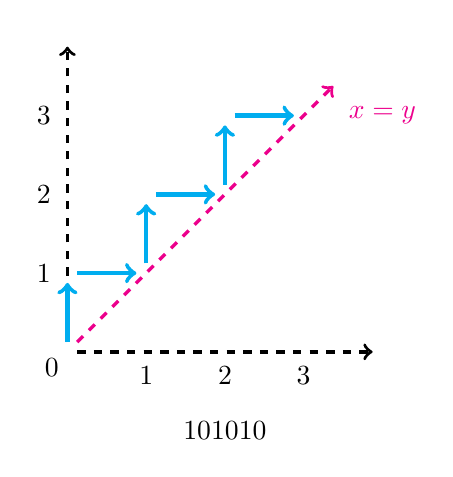
\begin{tikzpicture}[scale = 1]
    \node (a) at (0, 0) {};
    \node (b) at (0, 4) {};
    \node (c) at (4, 0) {};
    \node (d) at (3.5, 3.5) {};
    \node (e) at (4, 3) [color = magenta]
        {$x = y$}; 
    \draw [dashed, very thick, ->] (a) to (b);
    \draw [dashed, very thick, ->] (a) to (c);
    \draw [dashed, very thick, ->]
        [color = magenta] (a) to (d);

    \node (1)  at (0,0)   {};
    \node (2)  at (0,1)   {};
    \node (3)  at (1,1)   {};
    \node (4)  at (1,2)   {};
    \node (5)  at (2,2)   {};
    \node (6)  at (2,3)   {};
    \node (7)  at (3,3)   {};
    \draw [->, ultra thick, color = cyan]
        (1)  to (2);
    \draw [->, ultra thick, color = cyan] 
        (2)  to (3);
    \draw [->, ultra thick, color = cyan]
        (3)  to (4);
    \draw [->, ultra thick, color = cyan]
        (4)  to (5);
    \draw [->, ultra thick, color = cyan]
        (5)  to (6);
    \draw [->, ultra thick, color = cyan]
        (6)  to (7);

    \node at (-0.2, -0.2) {$0$};
    \node at (-0.3, 1)    {$1$};
    \node at (1, -0.3)    {$1$};
    \node at (-0.3, 2)    {$2$};
    \node at (2, -0.3)    {$2$};
    \node at (-0.3, 3)    {$3$};
    \node at (3, -0.3)    {$3$};
    \node at (2, -1)      {$101010$};

\end{tikzpicture}
        Il y a $7^1 = 7$ éléments dans chacun de ces posets.
    \end{center}
\end{expl}

Ceci conclut la présentation de nos posets bijectifs.\\

Nous passons maintenant au second problème traité par cet article, à savoir
l'extension de la notion d'arbre de parking au cas rationnel.
En effet, définie par B. Delcroix-Oger, M. Josuat-Vergès et L. Randazzo
(2020), la structure d'arbre de parking (classique) est définie par une
bijection avec les fonctions de parking classiques.
Nous définissons donc les arbres de parking rationnels, extension qui sera,
similairement, en bijection avec les fonctions de parking rationnelles.